\chapter{Preparing Climate Data with R in Colab}

Welcome to the practical side of data analysis! In Chapter 1, we explored the power of R packages. Now, we’ll apply that knowledge to a real-world scenario: working with climate data. Climate data, like weather station readings (temperature, precipitation, etc.), is fascinating but often comes with imperfections. It might have missing measurements, incorrect values, or inconsistent formats.

Before we can analyze data and draw meaningful conclusions, we must clean and preprocess it. This means identifying and fixing errors, handling missing information, and transforming the data into a suitable format for analysis. Think of it like preparing your ingredients before cooking – essential for a good final result!

In this chapter, we’ll use Google Colaboratory (Colab), a free, cloud-based platform that lets you write and run code (including R!) directly in your web browser. This is fantastic because you don’t need to install complex software on your own computer, and you can easily save and share your work.

\section{Setting Up Your Colab Environment for R}

Google Colab primarily supports Python, but we can easily configure it to run R code. To set up R environment we can perform following steps:

\begin{enumerate}
    \item \textbf{Access Google Colab:} Open your web browser and go to \url{https://colab.research.google.com}. You’ll need a Google account to use it.
    \item \textbf{Create a New Notebook:} Click on \texttt{File} $\rightarrow$ \texttt{New notebook}. This creates a new, empty Colab notebook file (which is automatically saved to your Google Drive). Rename it something descriptive, like ``Climate Dataset Analysis.''
    \item \textbf{Understanding the Interface:}
    \begin{itemize}
        \item \textbf{Cells:} Colab notebooks are made of cells. You’ll use Code cells to write and run R code and Text cells to add notes and explanations using Markdown.
        \item \textbf{Runtime:} This is the virtual machine in the cloud running your code.
        \item \textbf{Running Cells:} To run a cell, click the play button to its left or press \texttt{Shift + Enter}.
    \end{itemize}
    \item \textbf{Change Runtime to R:}
    \begin{itemize}
        \item Click \texttt{Runtime} on the menu.
        \item Choose \texttt{Change runtime type}.
        \item In the dropdown under ``Language,'' select \texttt{R}.
        \item Click \texttt{Save}.
    \end{itemize}
    \item \textbf{Installing Packages:} As shown in the setup cell, you install R packages in Colab just like you would locally, using \texttt{install.packages("package name")}. Any packages you install will be available for your current session but might need reinstalling if the runtime fully resets after a long period of inactivity.
\end{enumerate}

\section{Getting Climate Data into Colab}

Now we need some reliable data to conduct meaningful analysis. In this chapter, we will work with climate data from Nepal, covering the period from 1980 to 2019. This dataset includes important environmental indicators such as temperature, precipitation, and humidity, which will help us explore climate trends over time.

\subsection*{Where to Find Climate Data:}

The dataset used in this chapter is publicly available on the Kaggle platform, a popular repository for datasets and data science projects. The dataset contains climate data for Nepal, including various meteorological parameters. These data were sourced from the NASA Langley Research Center (LaRC) POWER Project, which is funded through the NASA Earth Science/Applied Science Program. The data was extracted via NASA’s Power Access API. The information is based on measurements from 93 weather stations across 62 districts in Nepal, providing a comprehensive view of the country’s climate. We will import the required dataset directly from Kaggle. Make sure you have a Kaggle account.

You can view or download the dataset using the following link:

\medskip

\href{https://www.kaggle.com/code/saimondahal/nepal-climate-data-eda-insights/input}{Click here to access the dataset on Kaggle
}
\medskip

\subsection*{Loading Dataset in Colab:}

The dataset that we downloaded is in \texttt{.csv} format. We can rename the downloaded dataset as \texttt{dailyclimate.csv}. There are many ways to load the dataset in the Colab environment.
\begin{enumerate}
\item {Uploading Directly (Best for small files, $<$ 25MB)}  
    \begin{itemize}
        \item Click the folder icon in the left sidebar of Colab.
        \item Click the ``Upload'' button.
        \item Select your \texttt{weather data raw.csv} file from your computer.
    \end{itemize}
\noindent \textit{Note: Files uploaded this way disappear when the runtime restarts.}

\item {Mounting Google Drive (Recommended for larger/persistent files)}  
For this you must have the \texttt{dailyclimate.csv} in your Google Drive. Place your \texttt{dailyclimate.csv} file somewhere convenient in your Google Drive (e.g., in a folder called \texttt{Colab Data}).

    \begin{itemize}
        \item Click the folder icon in the left sidebar.
        \item Click the ``Mount Drive'' button (looks like a Google Drive logo).
        \item Follow the prompts in the popup window and the new code cell that appears. You’ll need to authorize Colab to access your Google Drive.
        \item Once mounted, your Google Drive files will appear under \texttt{/content/drive/MyDrive/}. You can navigate this like any other folder system.
    \end{itemize}
\end{enumerate}
We have successfully loaded the dataset in our Colab environment and now we can begin our data preparation for analysis.

\section{First Look - Exploring Your Climate Data}

Before cleaning, we need to understand our raw data. What does it look like? What kind of information does it contain? Are there obvious problems?

\subsection{Loading the Data into R}

Assuming you have the file available (either uploaded or on Drive), load it using \texttt{readr} (part of the tidyverse).

\begin{verbatim}
library(tidyverse)

# Path if mounted on Google Drive:
file_path <- "/content/drive/MyDrive/Colab_Data/dailyclimate.csv"

# Load the data
climate_data <- read.csv(file_path)

# Quick check
head(climate_data) # Display the first 6 rows
\end{verbatim}

\subsection{Dataset Dimension}

\begin{verbatim}
dim(climate_data)
\end{verbatim}
Dimension: 883,128 rows $\times$ 23 columns.

The dataset has 883,128 rows and 23 columns.

\subsection{Dataset Structure}

Understanding the structure of the dataset is essential before proceeding to cleaning. In R, we can use the below function to inspect the dataset.

\begin{verbatim}
str(climate_data)
\end{verbatim}

% Figure here ----------------------------
\begin{figure}[h!]
    \centering
    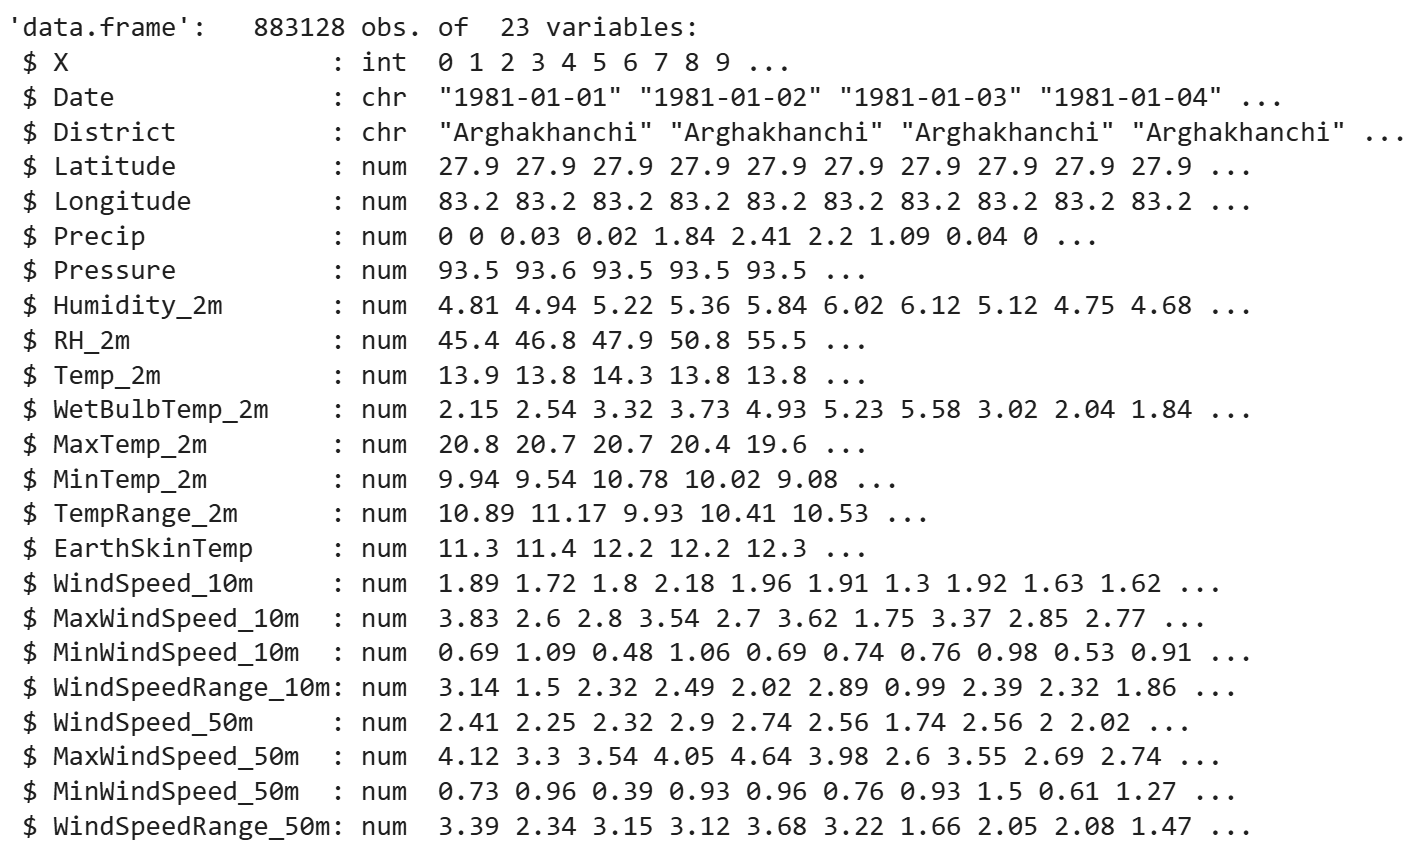
\includegraphics[width=0.7\textwidth]{figures/raw.png}
    \caption{Structure of the Climate Dataset.}
\end{figure}

\subsection{Data Summary}

The \texttt{summary()} function in R provides a quick statistical summary of each column in the dataset. It includes descriptive statistics like mean, median, minimum, maximum, and quartiles. It also shows missing values (NA) and category counts for factors.

\begin{verbatim}
summary(climate_data)
\end{verbatim}

% Figure here----------------------------
\begin{figure}[h!]
    \centering
     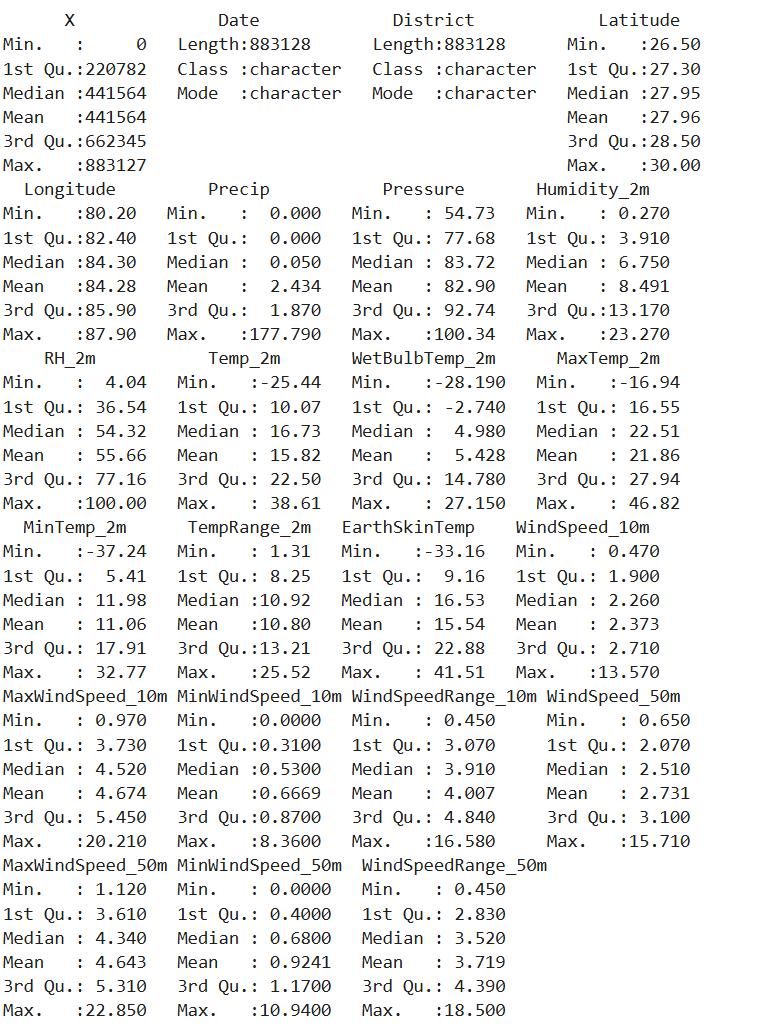
\includegraphics[width=0.5\textwidth]{figures/summary.png}
    \caption{Summary of the Climate Dataset.}
\end{figure}

\subsubsection*{What to Look for During Exploration:}

\begin{enumerate}
    \item \textbf{Data Types:} Are dates recognized as dates? Are numeric values (like temperature) stored as numbers or text?
    \item \textbf{Missing Values (NA):} How many missing values are there in each column (\texttt{summary()} is great for this)?
    \item \textbf{Ranges:} Do minimum and maximum values make sense (\texttt{summary()})? (e.g., Temperatures shouldn’t be -200°C, precipitation shouldn’t be negative).
\end{enumerate}

\section{Data Preprocessing}

Data preprocessing is the process of preparing raw data for analysis by cleaning and transforming it into a usable format. In data mining it refers to preparing raw data for mining by performing tasks like cleaning, transforming, and organizing it into a format suitable for mining algorithms.

Goal is to improve the quality of the data, handling missing values, removing duplicates, and normalizing data to ensures the accuracy and consistency of the dataset.

\subsection{Data Cleaning}

In this step, we focus on cleaning the dataset to prepare it for analysis.

\begin{enumerate}
\item \textbf{Check For Null Values:}

We should identify any missing values across the dataset, and decide how to handle them (impute, drop, or analyze separately). For this particular dataset no null values were found.

\begin{verbatim}
sum(is.na(df_climate))
\end{verbatim}

\item\textbf{Drop the unnecessary columns:}

In our data set the first column consisting of an index is not necessary so we can drop the first unnamed column from our climate dataset.

\begin{verbatim}
df_climate$X <- NULL
\end{verbatim}

\item\textbf{Inspect the Duplicate Columns:}

We must also check for duplicate columns and remove them as they don't provide any additional information. For this particular climate dataset no such columns were found.

\begin{verbatim}
duplicated(colnames(df_climate))
\end{verbatim}

\item\textbf{Convert Date Column to Date Format:}

Since the Date column is currently in character format, convert it to Date using \texttt{as.Date()}.

\begin{verbatim}
df_climate$Date <- as.Date(df_climate$Date, format = "%Y-%m-%d")
\end{verbatim}

\item \textbf{Set Date as Index:}

Setting the date as an index is not strictly necessary in R for time series data analysis, but it is often a good practice and can simplify time-based operations. Setting the date as an index (or primary column) helps in slicing, filtering, and aggregating data by time periods. For this data set I used \texttt{tsibble} package.

\begin{verbatim}
# Convert tibble to tsibble
df_climate <- as_tsibble(df_climate, index = Date, key = District)

# Check for index
index_name <- index_var(df_climate)
print(index_name)
\end{verbatim}

The dataset structure after cleaning looks like:

\begin{verbatim}
glimpse(df_climate)
\end{verbatim}

% Figure here ---------------------------
\begin{figure}[h!]
    \centering
    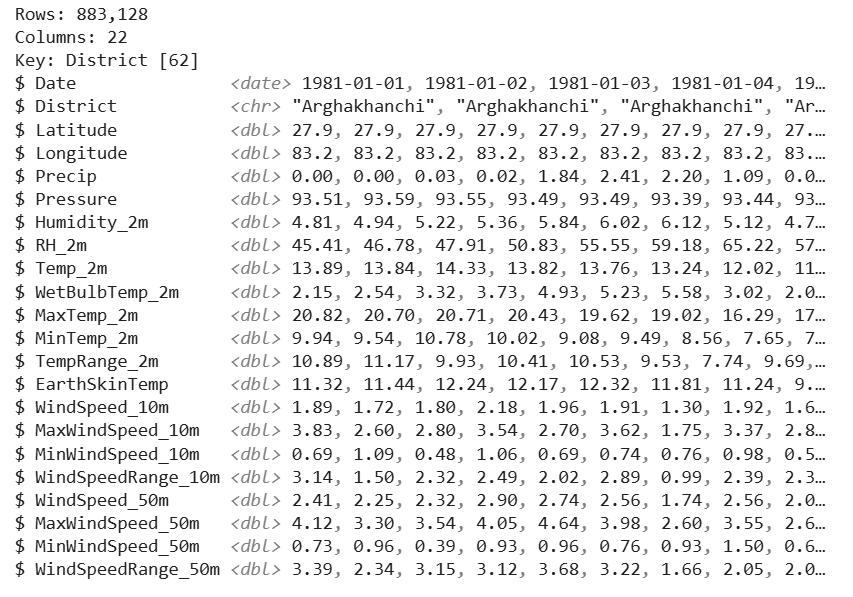
\includegraphics[width=0.6\textwidth]{figures/glimpse.png}
    \caption{Glimpse of the Cleaned Climate Dataset.}
\end{figure}

\end{enumerate}
\subsection{Feature Engineering}

Feature engineering is the process of taking raw data and transforming it into meaningful inputs that help a machine learning model understand patterns better. Think of it like preparing ingredients before cooking like when you chop, mix, and season them so the final dish tastes great.

In data analysis, this means creating new variables, cleaning data, selecting important information, or combining features to improve the model’s ability to make accurate predictions. Good feature engineering can often make a bigger difference in model performance than just using more complex algorithms.

It helps to create new features that might be helpful for your analysis. For this dataset, we can derive the month column from Date. Since Date is in format YYYY-MM-DD, we can extract the month and create a new column called month number. We can also create another column called month label and assign the names of the month (e.g., 1 = Jan, 2 = Feb, and so on).

\begin{verbatim}
# Extract month as number and label
df_climate$Month_Number <- month(df_climate$Date)     
df_climate$Month_Label <- month(df_climate$Date, label = TRUE)
\end{verbatim}

We can categorize the months into season and create a new column called “Season” for seasonal data analysis in the following way:

\begin{verbatim}
# Categorize months into seasons
df_climate <- df_climate %>%
  mutate(Season = case_when(
    month(Date) %in% c(12, 1, 2)  ~ "Winter",
    month(Date) %in% c(3, 4, 5)   ~ "Spring",
    month(Date) %in% c(6, 7, 8)   ~ "Summer",
    month(Date) %in% c(9, 10, 11) ~ "Fall"
  ))
\end{verbatim}

In R we can use \texttt{dplyr} and \texttt{lubridate} to extract the components of date. The function called \texttt{mutate()} can be used for creation of new columns and modifying the existing columns in our case.
